\documentclass[11pt,a4paper]{article}

% Image mode: pdf.
% Image paths stay relative. In PDF mode, place same-basename PDF conversions
% of the chapter SVG files in the assets/ directory beside this source.

\usepackage{iftex}
\ifPDFTeX
  \PackageError{handout}{This template requires XeTeX or Tectonic}{Compile with xelatex or tectonic.}
\fi

\usepackage[a4paper,top=18mm,bottom=20mm,left=20mm,right=20mm,headsep=6mm]{geometry}
\usepackage{fontspec}
\usepackage{xeCJK}
\usepackage{amsmath}
\usepackage{unicode-math}

% Font settings are intentionally visible in the generated .tex file.
% These defaults target the macOS machine used for the released PDF.
% Change the family names when compiling on another system.
\setmainfont{Songti TC}
\setsansfont{Heiti TC}
\setmonofont{Menlo}
\setCJKmainfont{Songti TC}
\setCJKsansfont{Heiti TC}
\setCJKmonofont{Heiti TC}
\setmathfont{STIX Two Math}
\XeTeXlinebreaklocale "zh"
\XeTeXlinebreakskip=0pt plus 1pt

\usepackage{xcolor}
\definecolor{HandoutBlue}{HTML}{215A91}
\definecolor{HandoutBlueLight}{HTML}{EEF5FC}
\definecolor{HandoutGreen}{HTML}{39715A}
\definecolor{HandoutGreenLight}{HTML}{EFF8F3}
\definecolor{HandoutGold}{HTML}{8A641C}
\definecolor{HandoutGoldLight}{HTML}{FFF8E8}
\definecolor{HandoutInk}{HTML}{253142}
\definecolor{HandoutMuted}{HTML}{667085}

\usepackage{graphicx}
\makeatletter
% Pandoc 3 emits an accessibility `alt` key for raster/PDF images. Older
% graphicx releases do not know that key, so accept it without changing layout.
\@ifundefined{KV@Gin@alt}{\define@key{Gin}{alt}{}}{}
\newsavebox\pandoc@box
\newcommand*\pandocbounded[1]{%
  \sbox\pandoc@box{#1}%
  \Gscale@div\@tempa{\textheight}{\dimexpr\ht\pandoc@box+\dp\pandoc@box\relax}%
  \Gscale@div\@tempb{\linewidth}{\wd\pandoc@box}%
  \ifdim\@tempb\p@<\@tempa\p@\let\@tempa\@tempb\fi
  \ifdim\@tempa\p@<\p@\scalebox{\@tempa}{\usebox\pandoc@box}%
  \else\usebox{\pandoc@box}%
  \fi
}
\makeatother
\usepackage{float}
\floatplacement{figure}{H}
% Pandoc uses LTcaptype=none for uncaptioned longtables. The caption package
% expects that name to exist as a counter even though it is never displayed.
\newcounter{none}
\usepackage{caption}
\captionsetup[figure]{labelformat=empty,labelsep=none,font=small}

\usepackage{booktabs,longtable,array,calc}
\usepackage{etoolbox}
\makeatletter
\patchcmd\longtable{\par}{\if@noskipsec\mbox{}\fi\par}{}{}
\makeatother

\usepackage[most]{tcolorbox}
\tcbuselibrary{breakable,skins}
\newtcolorbox{HandoutLearningMap}{
  enhanced,breakable,colback=HandoutBlueLight,colframe=HandoutBlue,
  boxrule=0.8pt,arc=1.5mm,left=3mm,right=3mm,top=2mm,bottom=2mm,
  before skip=8pt,after skip=10pt
}
\newtcolorbox{HandoutWorkedExample}{
  enhanced,breakable,colback=HandoutGreenLight,colframe=HandoutGreen,
  boxrule=0.65pt,arc=1.5mm,left=3mm,right=3mm,top=2mm,bottom=2mm,
  before skip=8pt,after skip=10pt
}
\newtcolorbox{HandoutSelfCheck}{
  enhanced,breakable,colback=HandoutGoldLight,colframe=HandoutGold,
  boxrule=0.65pt,arc=1.5mm,left=3mm,right=3mm,top=2mm,bottom=2mm,
  before skip=8pt,after skip=10pt
}

\usepackage{titlesec}
\titleformat{\section}{\sffamily\bfseries\Large\color{HandoutBlue}}{}{0pt}{}
\titleformat{\subsection}{\sffamily\bfseries\large\color{HandoutInk}}{}{0pt}{}
\titleformat{\subsubsection}{\sffamily\bfseries\normalsize\color{HandoutInk}}{}{0pt}{}
\titlespacing*{\section}{0pt}{1.4em}{0.55em}
\titlespacing*{\subsection}{0pt}{1.15em}{0.45em}
\titlespacing*{\subsubsection}{0pt}{0.9em}{0.35em}
\setcounter{secnumdepth}{-\maxdimen}

\usepackage{hyperref}
\usepackage{bookmark}
\IfFileExists{xurl.sty}{\usepackage{xurl}}{}
\urlstyle{same}
\hypersetup{
  colorlinks=true,
  linkcolor=HandoutBlue,
  urlcolor=HandoutBlue,
  citecolor=HandoutBlue,
  pdftitle={數2-4 三角比},
  pdfsubject={數學},
  pdfcreator={Pandoc with the HighSchooContent LaTeX template}
}

\setlength{\parindent}{0pt}
\setlength{\parskip}{0.55em plus 0.15em minus 0.1em}
\setlength{\emergencystretch}{3em}
\setlength{\LTpre}{0.5em}
\setlength{\LTpost}{0.5em}
\renewcommand{\arraystretch}{1.18}
\providecommand{\tightlist}{%
  \setlength{\itemsep}{0pt}\setlength{\parskip}{0pt}}
\pagestyle{plain}


\begin{document}

\begin{tcolorbox}[
  enhanced,colback=white,colframe=HandoutBlue,boxrule=1.1pt,arc=2mm,
  borderline west={3pt}{0pt}{HandoutBlue},left=5mm,right=4mm,top=4mm,bottom=4mm
]
{\sffamily\small\bfseries\color{HandoutBlue}學生講義}\par
{\sffamily\bfseries\LARGE\color{HandoutInk}數2-4 三角比}\par
\vspace{0.35em}{\large 從相似三角形與坐標定義建立三角測量、面積與解三角形的方法}\par
\vspace{0.45em}{\small\color{HandoutMuted}%
科目：數學
\quad 課程：普通高中數學 第二冊
\quad 版本：學生版｜核心＋理解
\quad 校訂：2026-08-29
}\par
\vspace{0.25em}{\small\color{HandoutMuted}範圍：114 學年度數學第二冊第 4 章；直角三角形邊角關係、廣義角與極坐標、面積公式、正弦定理與餘弦定理}\par
\end{tcolorbox}


\begin{HandoutLearningMap}

\subsection{本章問題與能力}\label{ux672cux7ae0ux554fux984cux8207ux80fdux529b}

\begin{enumerate}
\def\labelenumi{\arabic{enumi}.}
\tightlist
\item
  為何固定銳角後，直角三角形的三個邊長比不隨大小改變？
\item
  如何把正弦、餘弦、正切推廣到鈍角、負角與超過一圈的角？
\item
  直線斜角與極坐標如何用角度描述方向？
\item
  正射影與正弦如何把兩邊夾角轉成面積？
\item
  正弦定理、餘弦定理各適合哪些已知條件，SSA 為何可能有兩個三角形？
\end{enumerate}

本章路徑：相似邊比 → 廣義角坐標 → 方向表示 → 正射影與面積 → 解任意三角形。

\end{HandoutLearningMap}

\section{0. 本章實際用途：用角度取得難以直接量到的長度}\label{ux672cux7ae0ux5be6ux969bux7528ux9014ux7528ux89d2ux5ea6ux53d6ux5f97ux96e3ux4ee5ux76f4ux63a5ux91cfux5230ux7684ux9577ux5ea6}

三角比把方向與長度比例連在一起。知道水平距離與仰角，就能求建築高度；知道一段可測基線與兩端觀測角，就能定位河對岸、山頂或船隻。測量、導航、測繪、攝影定位及工程放樣都使用相同幾何機制。

坐標定義把三角比從直角三角形推廣到任意方向。單位圓上的點以 \((\cos\theta,\sin\theta)\) 表示方向，斜率是 \(\tan\theta\)，極坐標則用距離 \(r\) 與方向角 \(\theta\) 表示位置。這些表示法也會在向量、週期現象與物理分量中再次出現。

任意三角形的資料常只有三邊、兩邊夾角或一組對邊---對角。正弦定理與餘弦定理提供從已知資料還原其餘邊角的系統方法；選擇定理前先辨認已知資料的配對關係，可直接降低列式錯誤。

\section{1. 直角三角形的邊角關係}\label{ux76f4ux89d2ux4e09ux89d2ux5f62ux7684ux908aux89d2ux95dcux4fc2}

\subsection{1.1 三角比由相似三角形定義}\label{ux4e09ux89d2ux6bd4ux7531ux76f8ux4f3cux4e09ux89d2ux5f62ux5b9aux7fa9}

固定銳角 \(\theta\)，任取兩個含 \(\theta\) 的直角三角形。兩者都有直角與角 \(\theta\)，由 AA 判定互相相似，所以對應邊成比例。三角形整體放大 \(k\) 倍時，任兩邊的比值中 \(k\) 會約去，因此比值只由 \(\theta\) 決定。

\begin{figure}
\centering
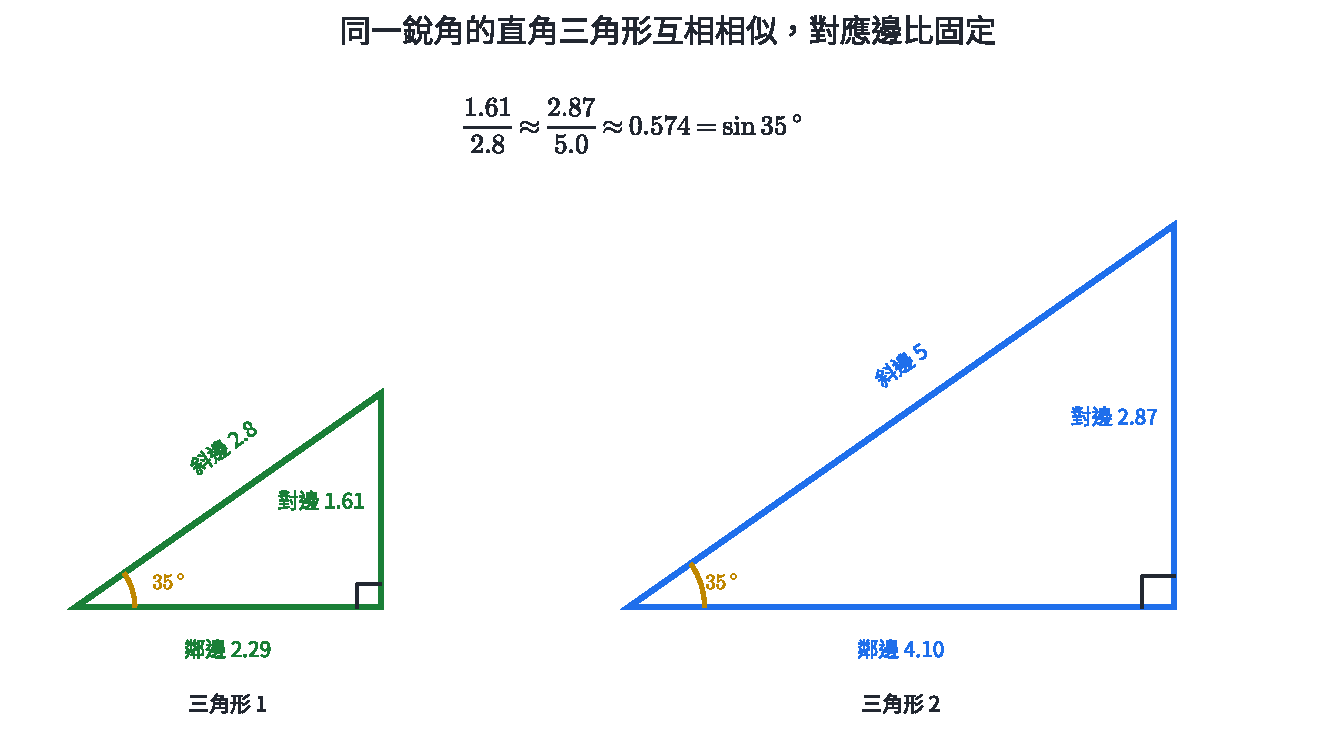
\includegraphics[width=0.9\linewidth,height=\textheight,keepaspectratio,alt={圖 1｜同一個銳角形成相似直角三角形，對應邊比不隨大小改變。}]{assets/數2-4-相似三角形邊比.pdf}
\caption{圖 1｜同一個銳角形成相似直角三角形，對應邊比不隨大小改變。}
\end{figure}

相對於銳角 \(\theta\)，直角對面的邊稱為斜邊，正對 \(\theta\) 的股稱為對邊，另一股稱為鄰邊。定義

\[
\boxed{\sin\theta=\frac{\text{對邊}}{\text{斜邊}}},\qquad
\boxed{\cos\theta=\frac{\text{鄰邊}}{\text{斜邊}}},\qquad
\boxed{\tan\theta=\frac{\text{對邊}}{\text{鄰邊}}}.
\]

三角比是長度相除所得的純數。由定義立即得到

\[
\boxed{\tan\theta=\frac{\sin\theta}{\cos\theta}}.
\]

直角三角形的兩銳角互餘。相對於 \(\theta\) 的對邊，就是相對於 \(90^\circ-\theta\) 的鄰邊，因此

\[
\boxed{\sin(90^\circ-\theta)=\cos\theta},\qquad
\boxed{\cos(90^\circ-\theta)=\sin\theta}.
\]

\subsection{1.2 特殊角與基本關係}\label{ux7279ux6b8aux89d2ux8207ux57faux672cux95dcux4fc2}

\(45^\circ\) 的值來自等腰直角三角形；\(30^\circ,60^\circ\) 的值來自正三角形對半切開。

\begin{figure}
\centering
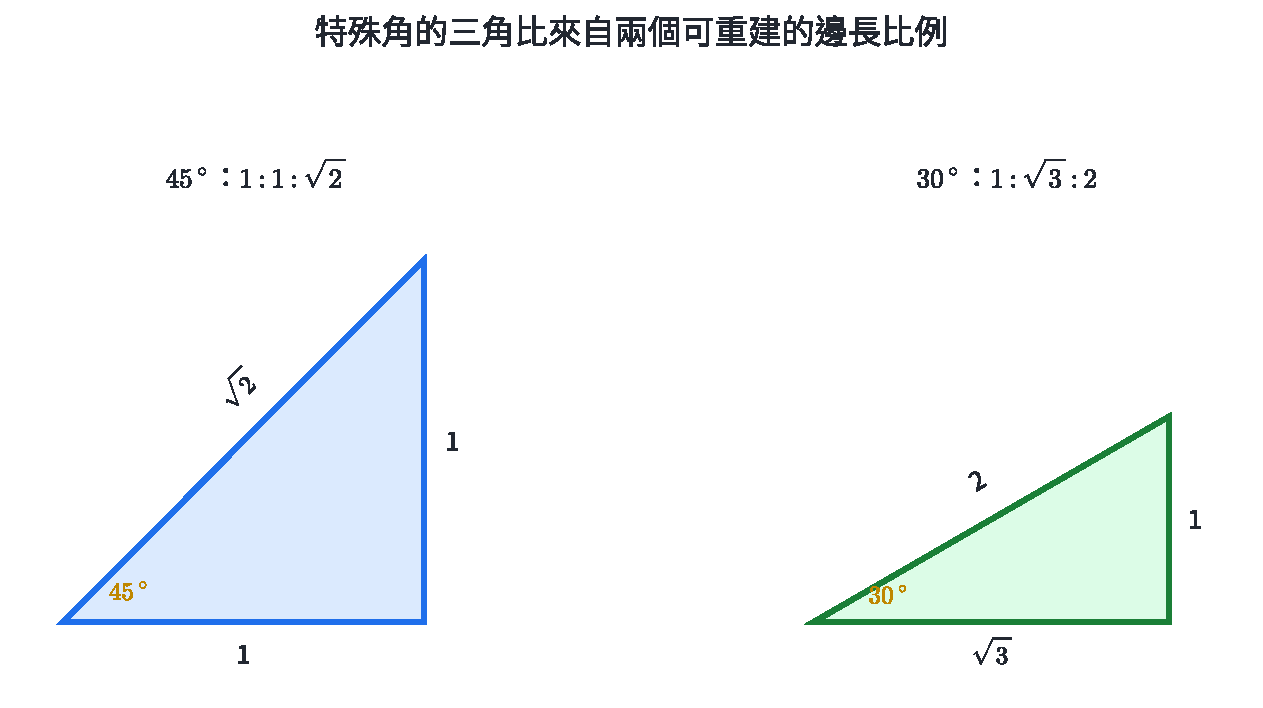
\includegraphics[width=0.88\linewidth,height=\textheight,keepaspectratio,alt={圖 2｜45\^{}\textbackslash circ 與 30\^{}\textbackslash circ 的三角比可由兩個特殊直角三角形重建。}]{assets/數2-4-特殊角三角形.pdf}
\caption{圖 2｜\(45^\circ\) 與 \(30^\circ\) 的三角比可由兩個特殊直角三角形重建。}
\end{figure}

{\def\LTcaptype{none} % do not increment counter
\begin{longtable}[]{@{}rrrr@{}}
\toprule\noalign{}
\(\theta\) & \(\sin\theta\) & \(\cos\theta\) & \(\tan\theta\) \\
\midrule\noalign{}
\endhead
\bottomrule\noalign{}
\endlastfoot
\(30^\circ\) & \(\dfrac12\) & \(\dfrac{\sqrt3}{2}\) & \(\dfrac{\sqrt3}{3}\) \\
\(45^\circ\) & \(\dfrac{\sqrt2}{2}\) & \(\dfrac{\sqrt2}{2}\) & \(1\) \\
\(60^\circ\) & \(\dfrac{\sqrt3}{2}\) & \(\dfrac12\) & \(\sqrt3\) \\
\end{longtable}
}

若直角三角形兩股為 \(a,b\)、斜邊為 \(c\)，畢氏定理給出

\[
\sin^2\theta+\cos^2\theta
=\frac{a^2}{c^2}+\frac{b^2}{c^2}=1.
\]

所以

\[
\boxed{\sin^2\theta+\cos^2\theta=1}.
\]

\subsection{1.3 計算機與反三角函數}\label{ux8a08ux7b97ux6a5fux8207ux53cdux4e09ux89d2ux51fdux6578}

一般角的三角比用計算機取得，本章角度單位使用 DEG。已知比值回推銳角時，使用 \(\sin^{-1},\cos^{-1},\tan^{-1}\)。例如

\[
\tan\theta=0.75
\quad\Rightarrow\quad
\theta=\tan^{-1}(0.75)\approx36.87^\circ.
\]

常見且會改變答案的兩項操作是角度模式與按鍵意義：DEG 與 RAD 的數值不同；\(\sin^{-1}x\) 表示反正弦，\(1/\sin x\) 才是倒數。

\subsection{例 1｜由三邊求銳角三角比}\label{ux4f8b-1ux7531ux4e09ux908aux6c42ux92b3ux89d2ux4e09ux89d2ux6bd4}

直角三角形兩股為 5、12，斜邊為 13。令 \(\theta\) 的對邊為 5，求三個三角比。

依定義

\[
\boxed{\sin\theta=\frac5{13}},\qquad
\boxed{\cos\theta=\frac{12}{13}},\qquad
\boxed{\tan\theta=\frac5{12}}.
\]

檢查：\((5/13)^2+(12/13)^2=1\)。

\subsection{例 2｜由仰角求建築高度}\label{ux4f8b-2ux7531ux4ef0ux89d2ux6c42ux5efaux7bc9ux9ad8ux5ea6}

觀測者眼睛離地 1.6 m，與建築底部的水平距離為 35 m，量得屋頂仰角 \(38^\circ\)。求建築高度。

令眼睛到屋頂的鉛直差為 \(h\)。直角三角形中

\[
\tan38^\circ=\frac{h}{35},
\]

所以

\[
h=35\tan38^\circ\approx27.35\text{ m}.
\]

加回眼高得建築高度

\[
\boxed{27.35+1.6\approx28.95\text{ m}}.
\]

\subsection{例 3｜已知三角比回推角度}\label{ux4f8b-3ux5df2ux77e5ux4e09ux89d2ux6bd4ux56deux63a8ux89d2ux5ea6}

一斜坡每水平前進 12 m 上升 5 m，求斜坡與水平面的夾角。

\[
\tan\theta=\frac5{12},\qquad
\theta=\tan^{-1}\!\left(\frac5{12}\right)\approx\boxed{22.62^\circ}.
\]

角度大小由上升量與水平量的比值決定，兩個長度同時放大時角度不變。

\subsubsection{練習 1A}\label{ux7df4ux7fd2-1a}

\begin{enumerate}
\def\labelenumi{\arabic{enumi}.}
\tightlist
\item
  直角三角形中，\(\theta\) 的對邊、鄰邊、斜邊依序為 8、15、17。求三個三角比。
\item
  求 \(\sin30^\circ+\cos60^\circ+\tan45^\circ\)。
\item
  已知 \(\cos\theta=12/13\) 且 \(\theta\) 為銳角，求 \(\sin\theta,\tan\theta\)。
\item
  梯子長 6 m，與地面夾角 \(65^\circ\)。梯頂離地多高？
\item
  樹影長 9.5 m，太陽仰角 \(52^\circ\)。忽略地面坡度，求樹高。
\item
  一條道路每水平 100 m 上升 8 m。求道路傾角，取到 \(0.1^\circ\)。
\end{enumerate}

\subsubsection{練習 1A 解析}\label{ux7df4ux7fd2-1a-ux89e3ux6790}

\begin{enumerate}
\def\labelenumi{\arabic{enumi}.}
\tightlist
\item
  \(\sin\theta=\boxed{8/17}\)、\(\cos\theta=\boxed{15/17}\)、\(\tan\theta=\boxed{8/15}\)。
\item
  \(1/2+1/2+1=\boxed{2}\)。
\item
  \(\sin\theta=\sqrt{1-(12/13)^2}=\boxed{5/13}\)，\(\tan\theta=(5/13)/(12/13)=\boxed{5/12}\)。
\item
  高度為 \(6\sin65^\circ\approx\boxed{5.44\text{ m}}\)。
\item
  \(h=9.5\tan52^\circ\approx\boxed{12.2\text{ m}}\)。
\item
  \(\theta=\tan^{-1}(8/100)\approx\boxed{4.6^\circ}\)。
\end{enumerate}

\section{2. 廣義角與坐標定義}\label{ux5ee3ux7fa9ux89d2ux8207ux5750ux6a19ux5b9aux7fa9}

\subsection{2.1 標準位置、同界角與參考角}\label{ux6a19ux6e96ux4f4dux7f6eux540cux754cux89d2ux8207ux53c3ux8003ux89d2}

把角的始邊放在 \(x\) 軸正向，逆時針旋轉定為正角，順時針旋轉定為負角。角可以超過一圈。終邊相同的角稱為同界角，所有同界角可寫成

\[
\boxed{\theta+360^\circ k},\qquad k\in\mathbb Z.
\]

終邊與 \(x\) 軸所形成的銳角稱為參考角。參考角提供三角比的絕對值，象限決定正負。

\subsection{2.2 終邊坐標定義}\label{ux7d42ux908aux5750ux6a19ux5b9aux7fa9}

在角 \(\theta\) 的終邊取非原點的點 \(P(x,y)\)，令

\[
r=\sqrt{x^2+y^2}>0.
\]

定義

\[
\boxed{\sin\theta=\frac yr},\qquad
\boxed{\cos\theta=\frac xr},\qquad
\boxed{\tan\theta=\frac yx}\quad(x\ne0).
\]

終邊上換一個點時，\(x,y,r\) 同比例縮放，三個比值保持不變。當 \(r=1\) 時，點落在單位圓上，坐標直接是

\[
\boxed{P=(\cos\theta,\sin\theta)}.
\]

\begin{figure}
\centering
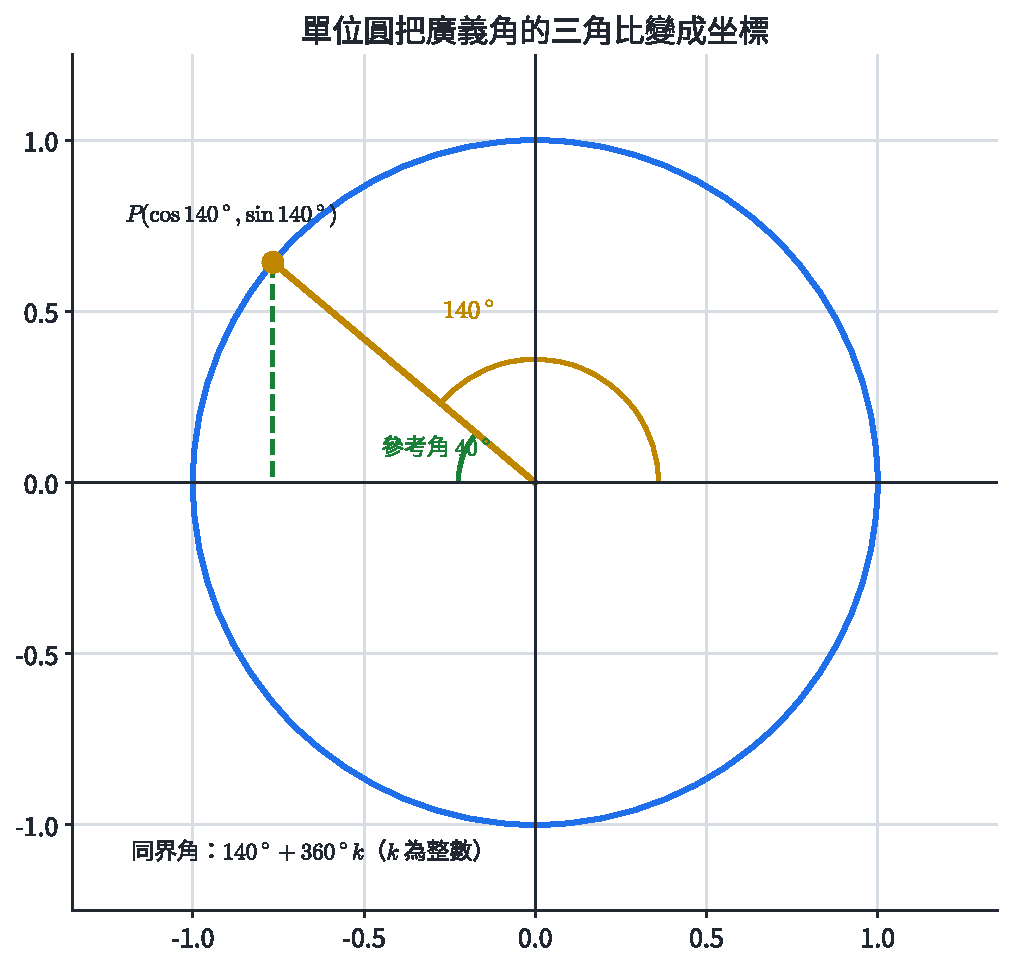
\includegraphics[width=0.84\linewidth,height=\textheight,keepaspectratio,alt={圖 3｜140\^{}\textbackslash circ 的終邊在第二象限，參考角為 40\^{}\textbackslash circ；單位圓坐標給出正弦與餘弦。}]{assets/數2-4-廣義角與單位圓.pdf}
\caption{圖 3｜\(140^\circ\) 的終邊在第二象限，參考角為 \(40^\circ\)；單位圓坐標給出正弦與餘弦。}
\end{figure}

\subsection{2.3 象限正負與平方關係}\label{ux8c61ux9650ux6b63ux8ca0ux8207ux5e73ux65b9ux95dcux4fc2}

因為 \(r>0\)，\(\sin\theta\) 的符號由 \(y\) 決定，\(\cos\theta\) 的符號由 \(x\) 決定，\(\tan\theta\) 的符號由 \(xy\) 是否同號決定。

{\def\LTcaptype{none} % do not increment counter
\begin{longtable}[]{@{}lrrr@{}}
\toprule\noalign{}
象限 & \(\sin\theta\) & \(\cos\theta\) & \(\tan\theta\) \\
\midrule\noalign{}
\endhead
\bottomrule\noalign{}
\endlastfoot
I & \(+\) & \(+\) & \(+\) \\
II & \(+\) & \(-\) & \(-\) \\
III & \(-\) & \(-\) & \(+\) \\
IV & \(-\) & \(+\) & \(-\) \\
\end{longtable}
}

坐標距離式 \(x^2+y^2=r^2\) 除以 \(r^2\)，得到對任意有定義的角皆成立的

\[
\boxed{\sin^2\theta+\cos^2\theta=1}.
\]

\begin{figure}
\centering
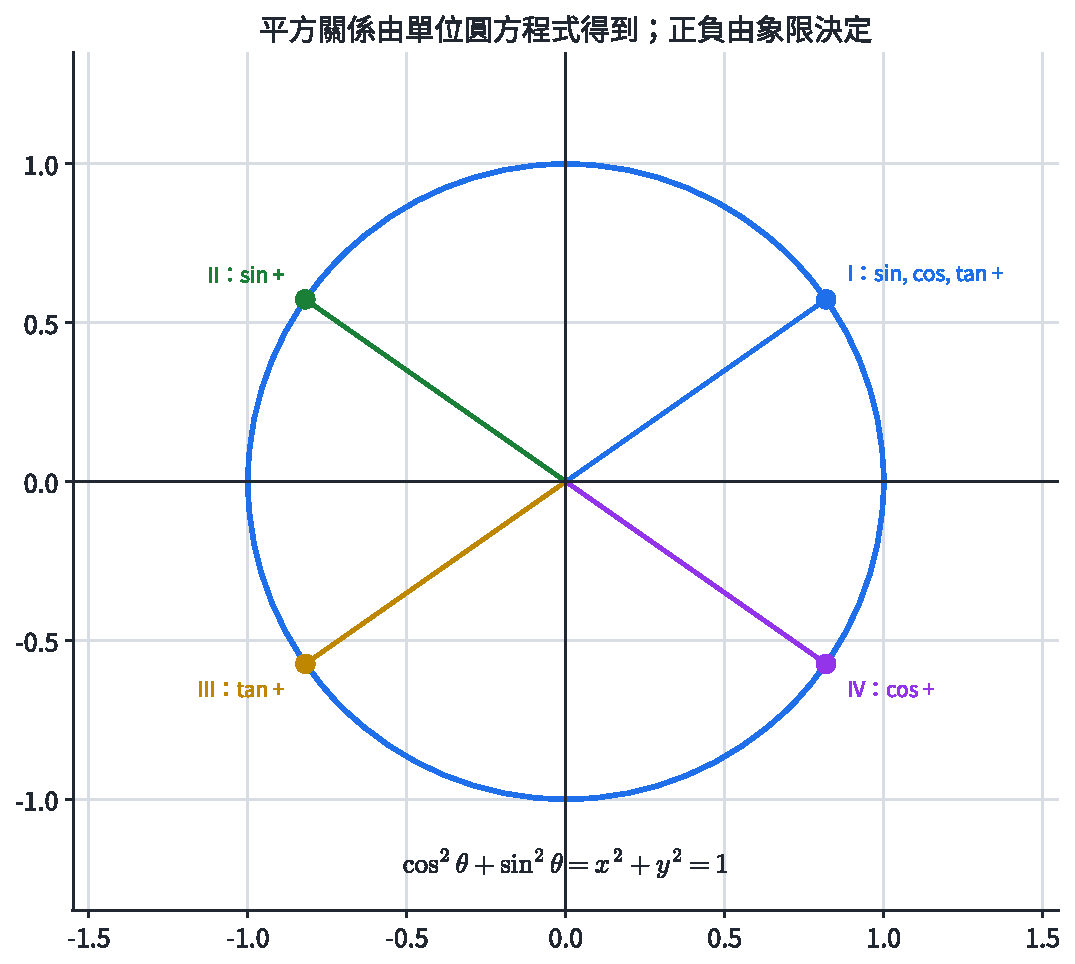
\includegraphics[width=0.84\linewidth,height=\textheight,keepaspectratio,alt={圖 4｜平方關係來自單位圓；開平方後的正負由終邊象限決定。}]{assets/數2-4-平方關係與象限.pdf}
\caption{圖 4｜平方關係來自單位圓；開平方後的正負由終邊象限決定。}
\end{figure}

象限軸角可由單位圓直接讀出：

{\def\LTcaptype{none} % do not increment counter
\begin{longtable}[]{@{}rrrrr@{}}
\toprule\noalign{}
\(\theta\) & \(0^\circ\) & \(90^\circ\) & \(180^\circ\) & \(270^\circ\) \\
\midrule\noalign{}
\endhead
\bottomrule\noalign{}
\endlastfoot
\(\sin\theta\) & \(0\) & \(1\) & \(0\) & \(-1\) \\
\(\cos\theta\) & \(1\) & \(0\) & \(-1\) & \(0\) \\
\(\tan\theta\) & \(0\) & 未定義 & \(0\) & 未定義 \\
\end{longtable}
}

\subsection{2.4 對稱角的三角比}\label{ux5c0dux7a31ux89d2ux7684ux4e09ux89d2ux6bd4}

單位圓上的坐標對稱直接給出三組基本關係。角 \(-\theta\) 的點是 \((\cos\theta,-\sin\theta)\)，因此

\[
\boxed{\sin(-\theta)=-\sin\theta},\qquad
\boxed{\cos(-\theta)=\cos\theta},\qquad
\boxed{\tan(-\theta)=-\tan\theta}.
\]

角 \(180^\circ-\theta\) 的點是 \((-\cos\theta,\sin\theta)\)，因此

\[
\boxed{\sin(180^\circ-\theta)=\sin\theta},
\]

\[
\boxed{\cos(180^\circ-\theta)=-\cos\theta},\qquad
\boxed{\tan(180^\circ-\theta)=-\tan\theta}.
\]

角 \(90^\circ-\theta\) 的點把兩坐標互換，因此

\[
\boxed{\sin(90^\circ-\theta)=\cos\theta},\qquad
\boxed{\cos(90^\circ-\theta)=\sin\theta}.
\]

例如已知 \(\sin\theta=0.7\)，則

\[
\cos(90^\circ+\theta)
=\cos\!\left(180^\circ-(90^\circ-\theta)\right)
=-\cos(90^\circ-\theta)
=\boxed{-0.7}.
\]

\subsection{例 4｜由終邊上一點求三角比}\label{ux4f8b-4ux7531ux7d42ux908aux4e0aux4e00ux9edeux6c42ux4e09ux89d2ux6bd4}

角 \(\theta\) 的終邊通過 \(P(-3,4)\)。求三個三角比並判斷象限。

\[
r=\sqrt{(-3)^2+4^2}=5.
\]

所以

\[
\boxed{\sin\theta=\frac45},\qquad
\boxed{\cos\theta=-\frac35},\qquad
\boxed{\tan\theta=-\frac43}.
\]

\(x<0,y>0\)，終邊在第二象限，三個符號與結果一致。

\subsection{例 5｜利用參考角求廣義角三角比}\label{ux4f8b-5ux5229ux7528ux53c3ux8003ux89d2ux6c42ux5ee3ux7fa9ux89d2ux4e09ux89d2ux6bd4}

求 \(\sin210^\circ,\cos210^\circ,\tan210^\circ\)。

\(210^\circ\) 在第三象限，參考角是 \(30^\circ\)。第三象限正弦、餘弦為負，正切為正：

\[
\boxed{\sin210^\circ=-\frac12},\quad
\boxed{\cos210^\circ=-\frac{\sqrt3}{2}},\quad
\boxed{\tan210^\circ=\frac{\sqrt3}{3}}.
\]

\subsection{例 6｜由一個三角比與象限求其餘比值}\label{ux4f8b-6ux7531ux4e00ux500bux4e09ux89d2ux6bd4ux8207ux8c61ux9650ux6c42ux5176ux9918ux6bd4ux503c}

已知 \(\sin\theta=-12/13\)，且 \(\theta\) 終邊在第四象限。求 \(\cos\theta,\tan\theta\)。

第四象限的餘弦為正。由平方關係

\[
\cos\theta=\sqrt{1-\frac{144}{169}}=\frac5{13}.
\]

因此

\[
\boxed{\cos\theta=\frac5{13}},\qquad
\boxed{\tan\theta=-\frac{12}{5}}.
\]

\subsection{例 7｜找同界角與象限}\label{ux4f8b-7ux627eux540cux754cux89d2ux8207ux8c61ux9650}

把 \(-750^\circ\) 化為 \(0^\circ\le\theta<360^\circ\) 的同界角。

\[
-750^\circ+3(360^\circ)=330^\circ.
\]

所以標準範圍內的同界角為 \(\boxed{330^\circ}\)，在第四象限，參考角為 \(30^\circ\)。

\subsubsection{練習 2A}\label{ux7df4ux7fd2-2a}

\begin{enumerate}
\def\labelenumi{\arabic{enumi}.}
\tightlist
\item
  寫出與 \(125^\circ\) 同界的兩個正角與兩個負角。
\item
  判斷 \(-200^\circ\) 的標準範圍同界角、象限與參考角。
\item
  終邊通過 \((5,-12)\)，求三個三角比。
\item
  求 \(\sin150^\circ,\cos150^\circ,\tan150^\circ\)。
\item
  已知 \(\cos\theta=-8/17\) 且 \(\theta\) 在第三象限，求 \(\sin\theta,\tan\theta\)。
\item
  解 \(0^\circ\le\theta<360^\circ\) 中滿足 \(\sin\theta=\sqrt3/2\) 的角；並求 \(\cos(180^\circ-\theta)\) 的可能值。
\end{enumerate}

\subsubsection{練習 2A 解析}\label{ux7df4ux7fd2-2a-ux89e3ux6790}

\begin{enumerate}
\def\labelenumi{\arabic{enumi}.}
\tightlist
\item
  例如正角 \(\boxed{485^\circ,845^\circ}\)；負角 \(\boxed{-235^\circ,-595^\circ}\)。
\item
  \(-200^\circ+360^\circ=160^\circ\)，在第二象限，參考角 \(\boxed{20^\circ}\)。
\item
  \(r=13\)，所以 \(\sin\theta=\boxed{-12/13}\)、\(\cos\theta=\boxed{5/13}\)、\(\tan\theta=\boxed{-12/5}\)。
\item
  參考角 \(30^\circ\)、第二象限：\(\boxed{1/2,-\sqrt3/2,-\sqrt3/3}\)。
\item
  第三象限正弦為負，\(\sin\theta=-\sqrt{1-64/289}=\boxed{-15/17}\)，\(\tan\theta=\boxed{15/8}\)。
\item
  參考角為 \(60^\circ\)，正弦在第一、二象限為正，故 \(\boxed{60^\circ,120^\circ}\)。兩個角的餘弦分別為 \(1/2,-1/2\)；由 \(\cos(180^\circ-\theta)=-\cos\theta\)，可能值仍為 \(\boxed{\pm1/2}\)。
\end{enumerate}

\section{3. 直線斜角與極坐標}\label{ux76f4ux7ddaux659cux89d2ux8207ux6975ux5750ux6a19}

\subsection{3.1 直線的斜角}\label{ux76f4ux7ddaux7684ux659cux89d2}

非鉛垂直線與 \(x\) 軸正向逆時針所成的角 \(\theta\)，取 \(0^\circ\le\theta<180^\circ\)，稱為直線斜角。取直線上兩點，水平變化為 \(\Delta x\)、鉛直變化為 \(\Delta y\)，則

\[
\boxed{m=\frac{\Delta y}{\Delta x}=\tan\theta}.
\]

正斜率對應第一象限方向的銳斜角；負斜率對應第二象限方向的鈍斜角。鉛垂線的斜角為 \(90^\circ\)，此時正切與斜率皆未定義。

\subsection{3.2 極坐標}\label{ux6975ux5750ux6a19}

平面上一點可用到原點的距離 \(r\ge0\) 與方向角 \(\theta\) 表示，記作 \((r,\theta)\)。極坐標轉直角坐標：

\[
\boxed{x=r\cos\theta},\qquad
\boxed{y=r\sin\theta}.
\]

直角坐標轉極坐標時先算

\[
\boxed{r=\sqrt{x^2+y^2}},
\]

再由 \(x,y\) 的符號決定象限，配合 \(\tan\theta=y/x\) 求方向角。同一點可用 \((r,\theta+360^\circ k)\) 表示；原點的 \(r=0\)，方向角可任取。

\begin{figure}
\centering
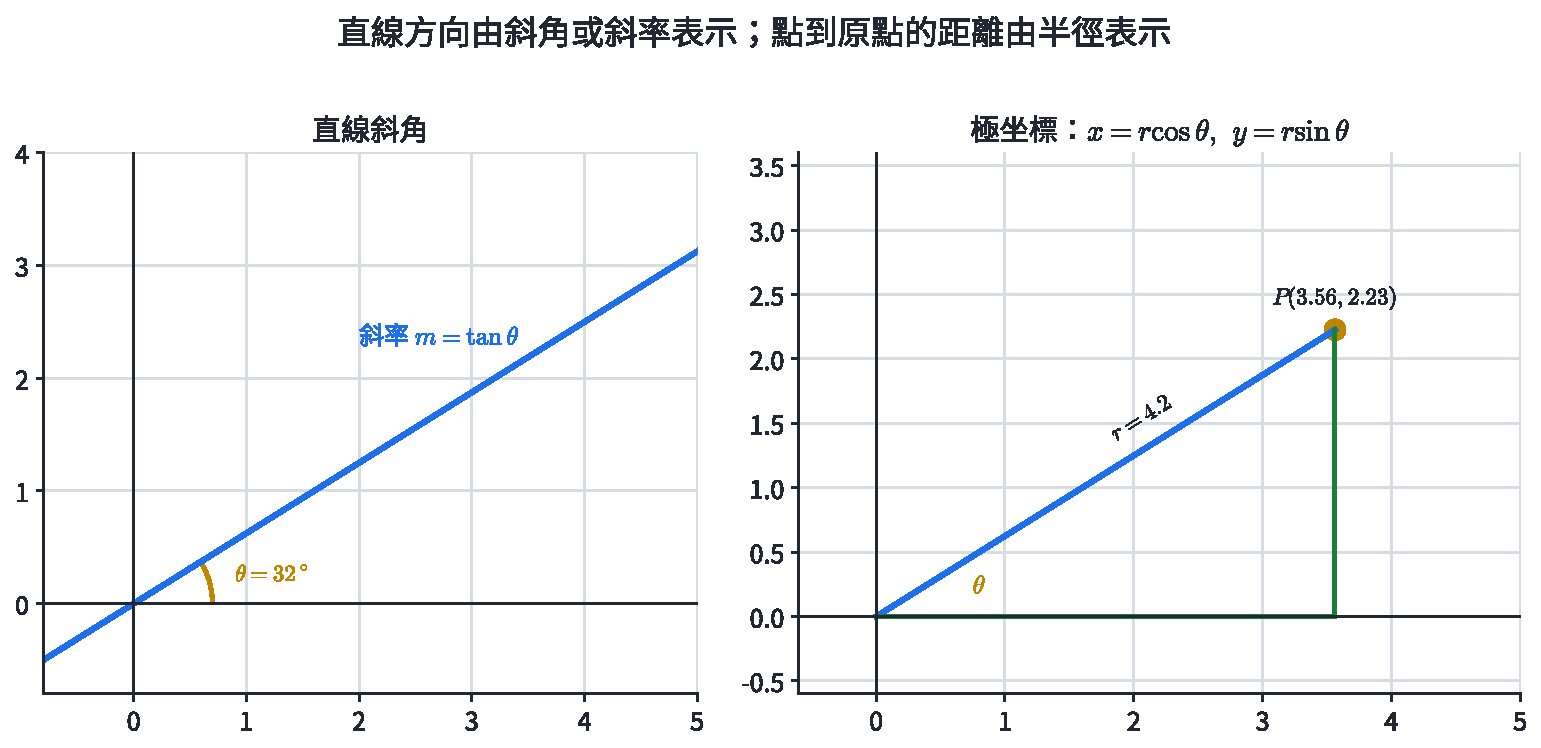
\includegraphics[width=0.94\linewidth,height=\textheight,keepaspectratio,alt={圖 5｜直線斜率與極坐標都以三角比把方向轉成坐標變化。}]{assets/數2-4-斜角與極坐標.pdf}
\caption{圖 5｜直線斜率與極坐標都以三角比把方向轉成坐標變化。}
\end{figure}

\subsection{例 8｜由斜率求直線斜角}\label{ux4f8b-8ux7531ux659cux7387ux6c42ux76f4ux7ddaux659cux89d2}

直線 \(3x-4y+8=0\) 化為 \(y=\frac34x+2\)，所以 \(m=3/4\)。

\[
\theta=\tan^{-1}\!\left(\frac34\right)\approx\boxed{36.87^\circ}.
\]

\subsection{例 9｜極坐標轉直角坐標}\label{ux4f8b-9ux6975ux5750ux6a19ux8f49ux76f4ux89d2ux5750ux6a19}

把 \((r,\theta)=(6,150^\circ)\) 轉成直角坐標。

\[
x=6\cos150^\circ=-3\sqrt3,\qquad
y=6\sin150^\circ=3.
\]

答案為 \(\boxed{(-3\sqrt3,3)}\)。

\subsection{例 10｜直角坐標轉極坐標}\label{ux4f8b-10ux76f4ux89d2ux5750ux6a19ux8f49ux6975ux5750ux6a19}

把 \(P(-3,3\sqrt3)\) 轉成 \(r\ge0,0^\circ\le\theta<360^\circ\) 的極坐標。

\[
r=\sqrt{9+27}=6.
\]

點在第二象限，\(|y/x|=\sqrt3\) 的參考角為 \(60^\circ\)，所以 \(\theta=120^\circ\)。極坐標為 \(\boxed{(6,120^\circ)}\)。

\subsubsection{練習 3A}\label{ux7df4ux7fd2-3a}

\begin{enumerate}
\def\labelenumi{\arabic{enumi}.}
\tightlist
\item
  求斜率 \(1\)、\(-1\) 的直線斜角。
\item
  直線 \(x+\sqrt3y-2=0\) 的斜角為何？
\item
  把 \((4,210^\circ)\) 轉成直角坐標。
\item
  把 \((0,-5)\) 轉成標準範圍極坐標。
\item
  點的極坐標為 \((8,330^\circ)\)。求它在 \(x,y\) 方向的投影長。
\end{enumerate}

\subsubsection{練習 3A 解析}\label{ux7df4ux7fd2-3a-ux89e3ux6790}

\begin{enumerate}
\def\labelenumi{\arabic{enumi}.}
\tightlist
\item
  \(m=1\) 得 \(\boxed{45^\circ}\)；\(m=-1\) 且斜角在 \([0,180^\circ)\)，得 \(\boxed{135^\circ}\)。
\item
  \(y=-x/\sqrt3+2/\sqrt3\)，\(m=-\sqrt3/3\)，斜角為 \(\boxed{150^\circ}\)。
\item
  \(x=4(-\sqrt3/2)=-2\sqrt3\)、\(y=4(-1/2)=-2\)，故 \(\boxed{(-2\sqrt3,-2)}\)。
\item
  \(r=5\)，方向為負 \(y\) 軸，故 \(\boxed{(5,270^\circ)}\)。
\item
  \(x=8\cos330^\circ=\boxed{4\sqrt3}\)，\(y=8\sin330^\circ=\boxed{-4}\)。
\end{enumerate}

\section{4. 正射影與三角形面積}\label{ux6b63ux5c04ux5f71ux8207ux4e09ux89d2ux5f62ux9762ux7a4d}

\subsection{4.1 正射影長}\label{ux6b63ux5c04ux5f71ux9577}

長度為 \(b\) 的線段與指定正向夾角為 \(C\)，它在該方向的帶號正射影為

\[
\boxed{b\cos C}.
\]

當 \(C\) 為銳角，投影與正向相同；當 \(C\) 為鈍角，\(\cos C<0\)，負號記錄投影方向相反。三角形中，從一邊沿另一邊方向分解，可得射影關係，例如

\[
\boxed{c=a\cos B+b\cos A}.
\]

\subsection{4.2 兩邊夾角面積公式}\label{ux5169ux908aux593eux89d2ux9762ux7a4dux516cux5f0f}

若三角形兩邊為 \(a,b\)，夾角為 \(C\)，以 \(a\) 為底，對應高為 \(b\sin C\)，所以

\[
\boxed{K=\frac12ab\sin C}.
\]

輪換邊角可得

\[
\boxed{K=\frac12bc\sin A=\frac12ca\sin B=\frac12ab\sin C}.
\]

若已知三邊，可用\textbf{海龍公式}。令半周長

\[
s=\frac{a+b+c}{2},
\]

則

\[
\boxed{K=\sqrt{s(s-a)(s-b)(s-c)}}.
\]

它可由面積公式與餘弦定理推出。把

\[
K^2=\frac14a^2b^2(1-\cos^2C),
\qquad
\cos C=\frac{a^2+b^2-c^2}{2ab}
\]

合併並因式分解，得到

\[
16K^2=[(a+b)^2-c^2][c^2-(a-b)^2]
=16s(s-a)(s-b)(s-c).
\]

\begin{figure}
\centering
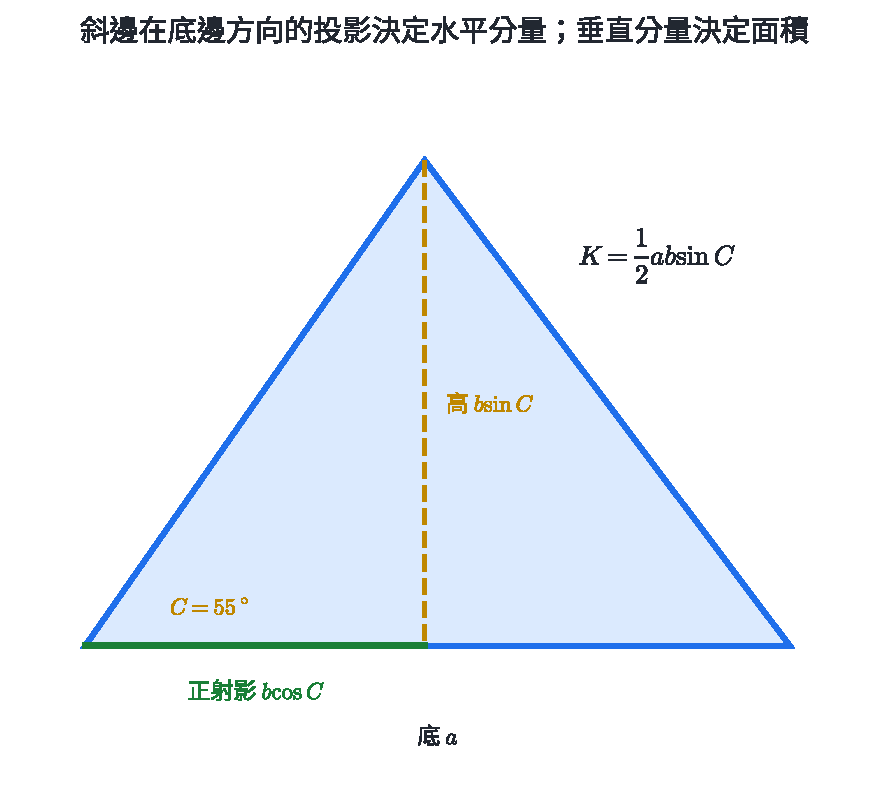
\includegraphics[width=0.91\linewidth,height=\textheight,keepaspectratio,alt={圖 6｜同一條斜邊的餘弦分量形成正射影，正弦分量形成高度。}]{assets/數2-4-正射影與面積.pdf}
\caption{圖 6｜同一條斜邊的餘弦分量形成正射影，正弦分量形成高度。}
\end{figure}

\subsection{例 11｜由兩邊夾角求面積}\label{ux4f8b-11ux7531ux5169ux908aux593eux89d2ux6c42ux9762ux7a4d}

三角形兩邊為 8、11，夾角 \(60^\circ\)。面積為

\[
K=\frac12(8)(11)\sin60^\circ
=44\cdot\frac{\sqrt3}{2}
=\boxed{22\sqrt3}.
\]

\subsection{例 12｜由面積反求夾角}\label{ux4f8b-12ux7531ux9762ux7a4dux53cdux6c42ux593eux89d2}

三角形兩邊為 10、13，面積為 52，且夾角 \(C\) 為銳角。求 \(C\)。

\[
52=\frac12(10)(13)\sin C,
\]

所以 \(\sin C=0.8\)。因 \(C\) 為銳角，

\[
C=\sin^{-1}(0.8)\approx\boxed{53.13^\circ}.
\]

\subsection{例 12-2｜由三邊求面積}\label{ux4f8b-12-2ux7531ux4e09ux908aux6c42ux9762ux7a4d}

三角形三邊為 13、14、15，半周長為

\[
s=\frac{13+14+15}{2}=21.
\]

由海龍公式

\[
K=\sqrt{21(21-13)(21-14)(21-15)}
=\sqrt{21\cdot8\cdot7\cdot6}
=\boxed{84}.
\]

\subsubsection{練習 4A}\label{ux7df4ux7fd2-4a}

\begin{enumerate}
\def\labelenumi{\arabic{enumi}.}
\tightlist
\item
  長 12 的線段與指定正向夾 \(30^\circ\)，求帶號投影長。
\item
  長 7 的線段與指定正向夾 \(120^\circ\)，求帶號投影長並解釋符號。
\item
  兩邊為 6、9，夾角 \(45^\circ\)，求三角形面積。
\item
  兩邊為 5、12，面積為 15，求夾角正弦值。
\item
  平行四邊形鄰邊為 8、13，夾角 \(70^\circ\)，求面積。
\item
  三角形三邊為 9、9、8，求面積。
\end{enumerate}

\subsubsection{練習 4A 解析}\label{ux7df4ux7fd2-4a-ux89e3ux6790}

\begin{enumerate}
\def\labelenumi{\arabic{enumi}.}
\tightlist
\item
  \(12\cos30^\circ=\boxed{6\sqrt3}\)。
\item
  \(7\cos120^\circ=\boxed{-3.5}\)；負號表示投影方向與指定正向相反。
\item
  \(K=\frac12(6)(9)\sin45^\circ=\boxed{27\sqrt2/2}\)。
\item
  \(15=\frac12(5)(12)\sin C\)，故 \(\boxed{\sin C=1/2}\)。
\item
  平行四邊形面積是同底同高三角形的兩倍，\(K=8(13)\sin70^\circ\approx\boxed{97.7}\)。
\item
  \(s=13\)，所以 \(K=\sqrt{13(4)(4)(5)}=\boxed{4\sqrt{65}}\)。
\end{enumerate}

\section{5. 正弦定理與餘弦定理}\label{ux6b63ux5f26ux5b9aux7406ux8207ux9918ux5f26ux5b9aux7406}

約定三角形 \(ABC\) 中，角 \(A,B,C\) 的對邊分別為 \(a,b,c\)。

\subsection{5.1 正弦定理}\label{ux6b63ux5f26ux5b9aux7406}

從 \(C\) 向 \(AB\) 作高 \(h\)。兩個直角三角形分別給出

\[
h=b\sin A=a\sin B.
\]

因此 \(a/\sin A=b/\sin B\)。對其他頂點重複同一推理，得到

\[
\boxed{\frac a{\sin A}=\frac b{\sin B}=\frac c{\sin C}=2R},
\]

其中 \(R\) 為外接圓半徑。正弦定理最直接的入口是已知一組「角與其對邊」。

\begin{figure}
\centering
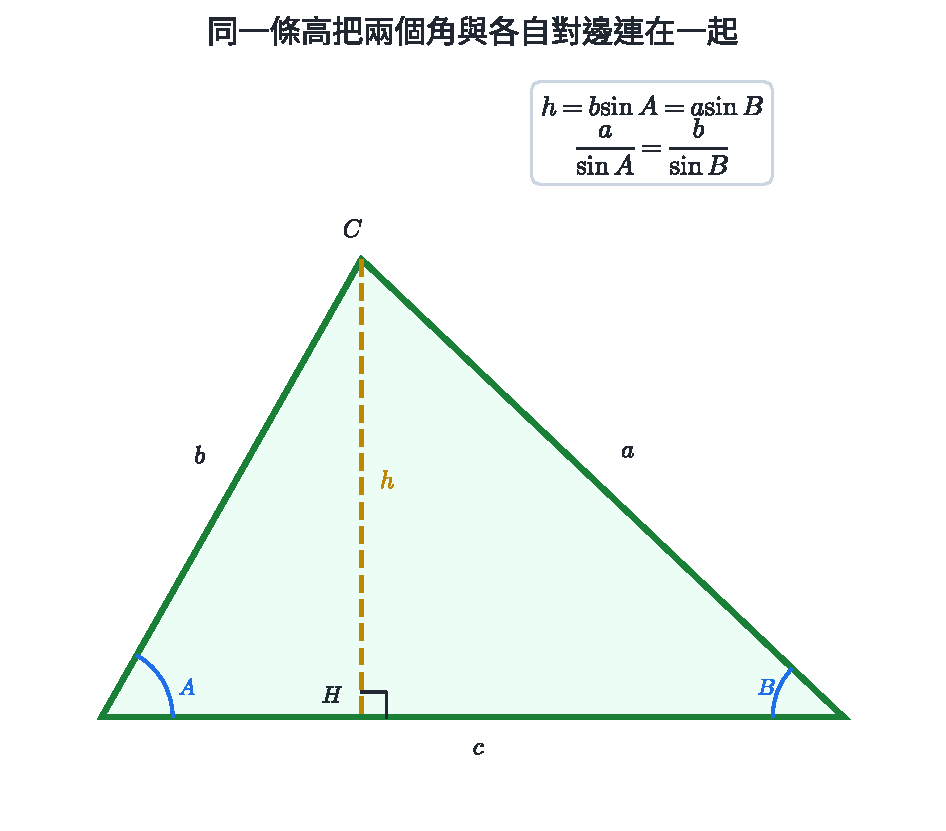
\includegraphics[width=0.9\linewidth,height=\textheight,keepaspectratio,alt={圖 7｜同一條高同時等於 b\textbackslash sin A 與 a\textbackslash sin B，推出正弦定理。}]{assets/數2-4-正弦定理推導.pdf}
\caption{圖 7｜同一條高同時等於 \(b\sin A\) 與 \(a\sin B\)，推出正弦定理。}
\end{figure}

\subsection{5.2 SSA 的解數}\label{ssa-ux7684ux89e3ux6578}

已知 \(A,a,b\) 時，正弦定理給出

\[
\sin B=\frac{b\sin A}{a}.
\]

當 \(A\) 為銳角，令高 \(h=b\sin A\)：

\begin{itemize}
\tightlist
\item
  \(a<h\)：0 解。
\item
  \(a=h\)：1 個直角三角形。
\item
  \(h<a<b\)：2 解。
\item
  \(a\ge b\)：1 解。
\end{itemize}

\begin{figure}
\centering
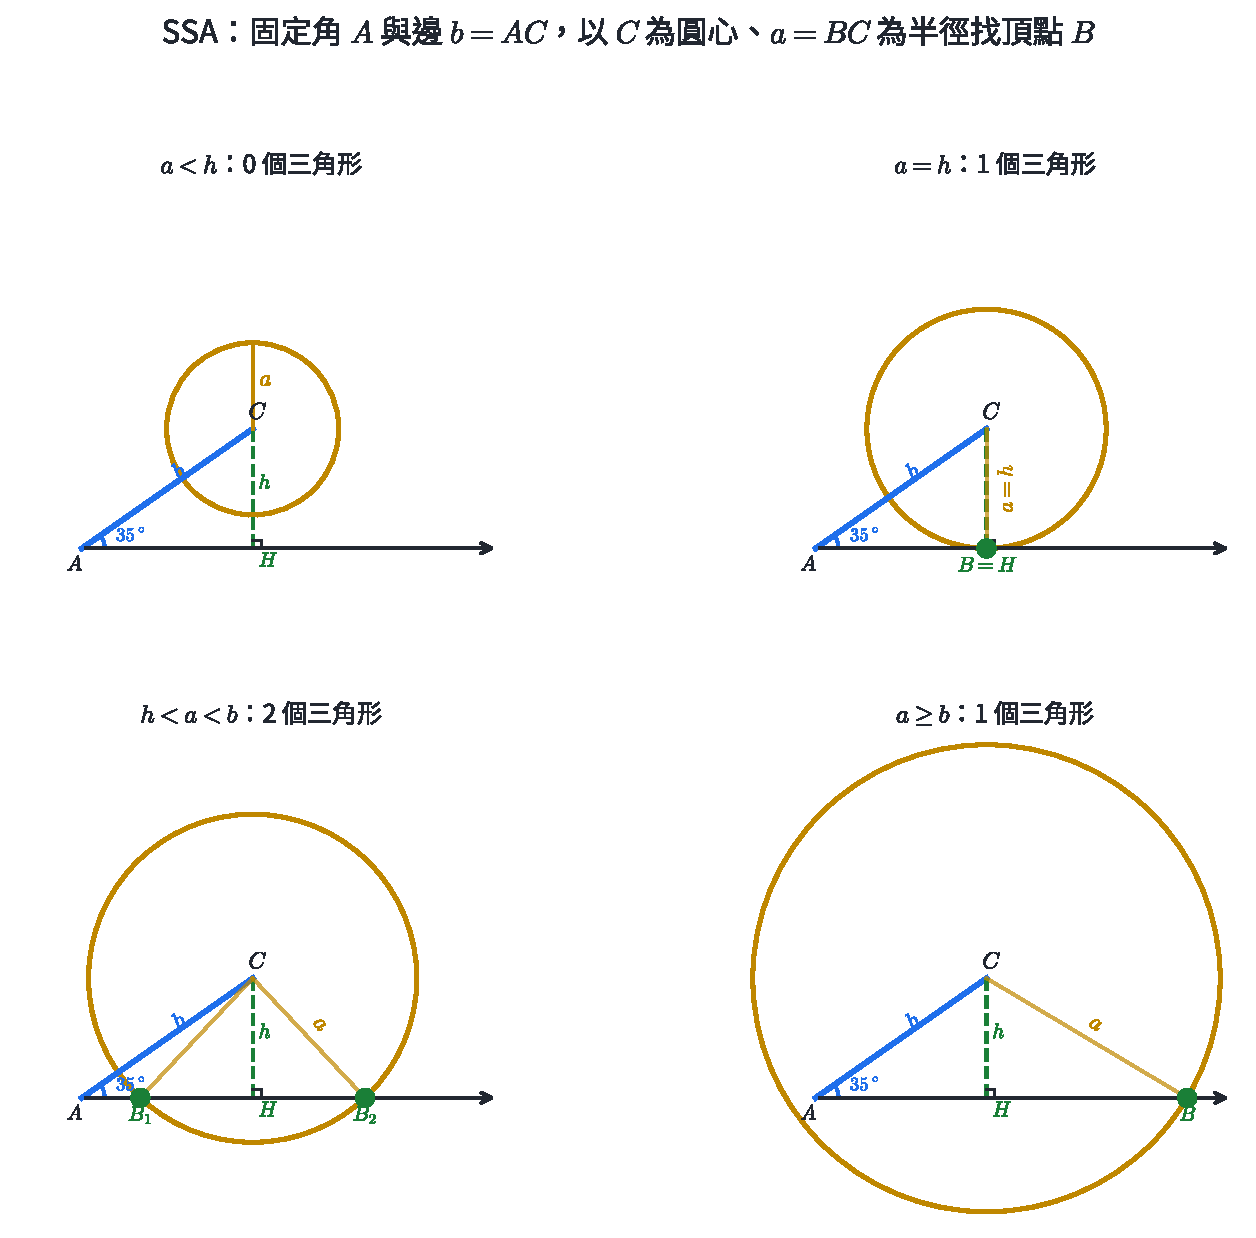
\includegraphics[width=0.96\linewidth,height=\textheight,keepaspectratio,alt={圖 8｜固定 A,b 後，以端點為圓心、半徑 a 與底邊的交點數就是三角形解數。}]{assets/數2-4-SSA解的個數.pdf}
\caption{圖 8｜固定 \(A,b\) 後，以端點為圓心、半徑 \(a\) 與底邊的交點數就是三角形解數。}
\end{figure}

計算時，若 \(0<\sin B<1\)，候選角為

\[
B_1=\sin^{-1}(u),\qquad B_2=180^\circ-B_1.
\]

逐一檢查 \(A+B<180^\circ\)，即可保留有效三角形。

\subsection{5.3 餘弦定理}\label{ux9918ux5f26ux5b9aux7406}

把角 \(C\) 放在原點，一邊端點設為 \((a,0)\)，另一邊端點設為 \((b\cos C,b\sin C)\)。兩端點距離為 \(c\)：

\[
\begin{aligned}
c^2
&=(a-b\cos C)^2+(b\sin C)^2\\
&=a^2+b^2-2ab\cos C.
\end{aligned}
\]

所以

\[
\boxed{c^2=a^2+b^2-2ab\cos C}.
\]

\begin{figure}
\centering
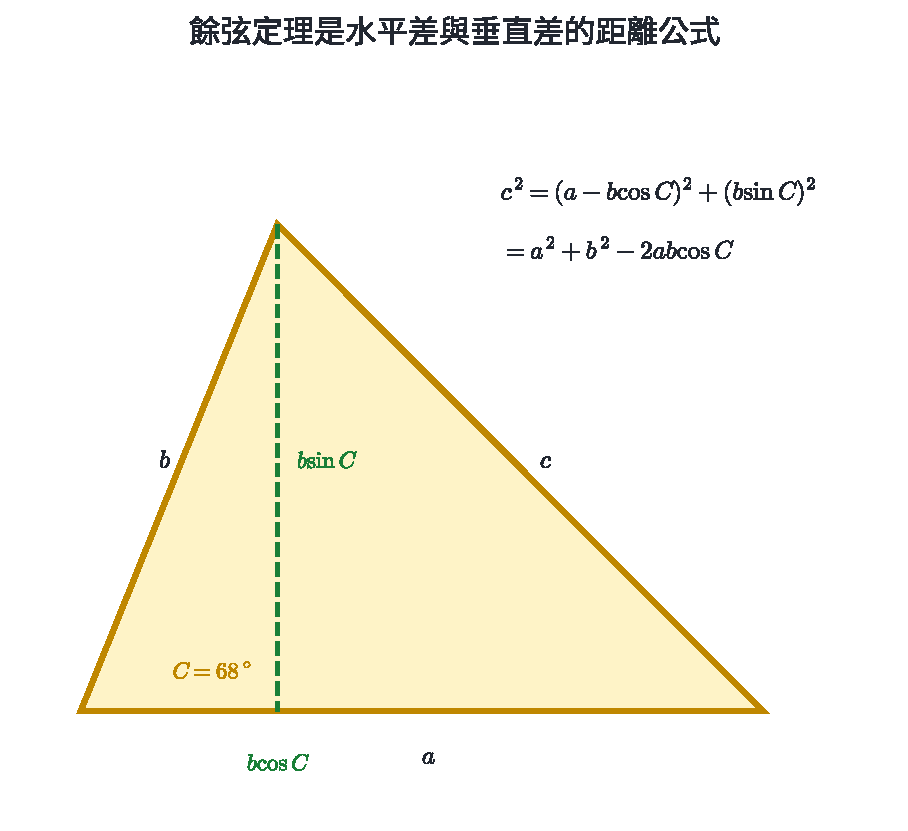
\includegraphics[width=0.89\linewidth,height=\textheight,keepaspectratio,alt={圖 9｜餘弦定理由水平差、垂直差與兩點距離公式直接推出。}]{assets/數2-4-餘弦定理坐標推導.pdf}
\caption{圖 9｜餘弦定理由水平差、垂直差與兩點距離公式直接推出。}
\end{figure}

已知三邊時可改寫為

\[
\boxed{\cos C=\frac{a^2+b^2-c^2}{2ab}}.
\]

若 \(C=90^\circ\)，\(\cos C=0\)，餘弦定理退化為畢氏定理。若 \(C\) 為鈍角，\(\cos C<0\)，因此對邊 \(c\) 的平方大於 \(a^2+b^2\)。

\subsection{5.4 基線三角測量}\label{ux57faux7ddaux4e09ux89d2ux6e2cux91cf}

選取兩個可到達點 \(A,B\)，量得基線 \(AB\) 與兩端指向目標 \(T\) 的角。三角形的第三角由內角和得到，再用正弦定理求 \(AT,BT\)。這種做法把難以直接測量的距離轉成一段可量基線與兩個方向角。

\begin{figure}
\centering
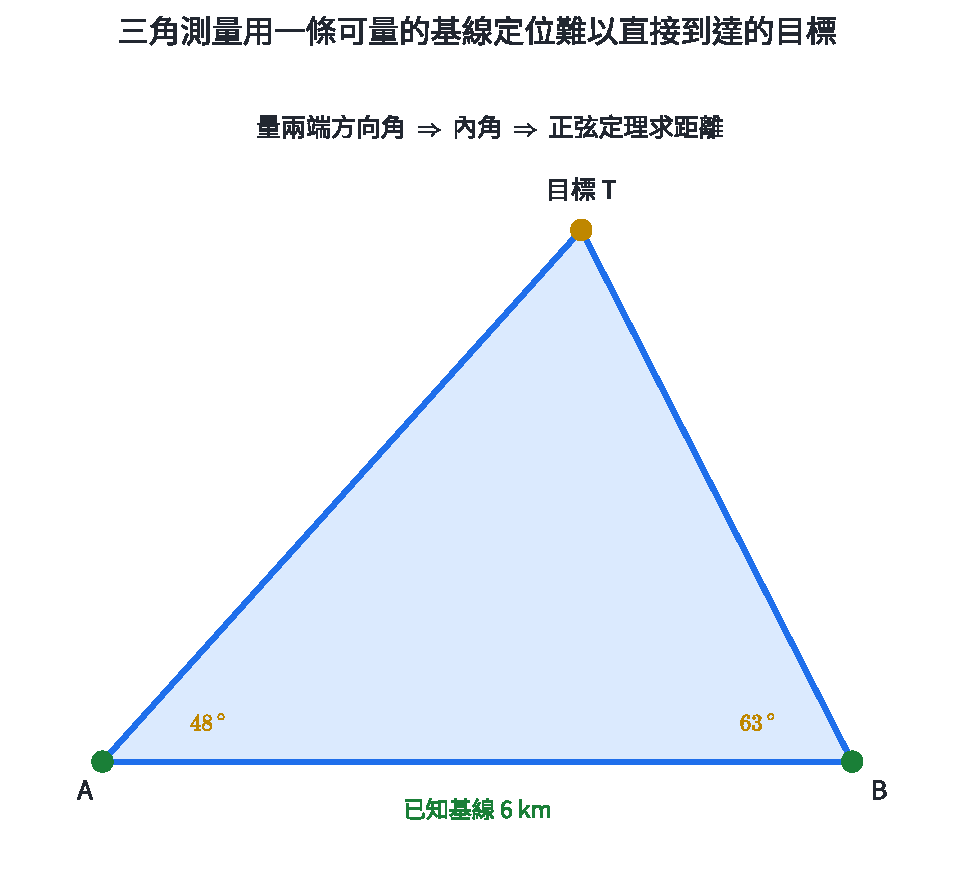
\includegraphics[width=0.91\linewidth,height=\textheight,keepaspectratio,alt={圖 10｜基線三角測量由一邊兩角定位遠端目標。}]{assets/數2-4-基線三角測量.pdf}
\caption{圖 10｜基線三角測量由一邊兩角定位遠端目標。}
\end{figure}

\subsection{例 13｜ASA 解三角形}\label{ux4f8b-13asa-ux89e3ux4e09ux89d2ux5f62}

已知 \(A=42^\circ,B=68^\circ,a=8\)。求 \(C,b,c\)。

\[
C=180^\circ-42^\circ-68^\circ=70^\circ.
\]

由正弦定理

\[
b=8\frac{\sin68^\circ}{\sin42^\circ}\approx\boxed{11.09},
\]

\[
c=8\frac{\sin70^\circ}{\sin42^\circ}\approx\boxed{11.24}.
\]

最大角 \(C=70^\circ\) 對應最大邊 \(c\)，與結果一致。

\subsection{例 14｜SSA 的兩個三角形}\label{ux4f8b-14ssa-ux7684ux5169ux500bux4e09ux89d2ux5f62}

已知 \(A=30^\circ,a=5,b=8\)。因

\[
h=b\sin A=8\cdot\frac12=4,
\]

且 \(4<5<8\)，所以有兩解。由正弦定理

\[
\sin B=\frac{8\sin30^\circ}{5}=0.8.
\]

因此

\[
B_1\approx53.13^\circ,\qquad B_2\approx126.87^\circ.
\]

兩者都滿足 \(A+B<180^\circ\)，對應

\[
C_1\approx96.87^\circ,\qquad C_2\approx23.13^\circ.
\]

\subsection{例 15｜SAS 用餘弦定理求第三邊}\label{ux4f8b-15sas-ux7528ux9918ux5f26ux5b9aux7406ux6c42ux7b2cux4e09ux908a}

已知 \(a=7,b=10,C=60^\circ\)。則

\[
c^2=7^2+10^2-2(7)(10)\cos60^\circ=79,
\]

所以 \(\boxed{c=\sqrt{79}\approx8.89}\)。

\subsection{例 16｜SSS 求角}\label{ux4f8b-16sss-ux6c42ux89d2}

三邊為 \(a=5,b=7,c=8\)。求角 \(C\)。

\[
\cos C=\frac{5^2+7^2-8^2}{2(5)(7)}=\frac17.
\]

所以

\[
C=\cos^{-1}\!\left(\frac17\right)\approx\boxed{81.79^\circ}.
\]

\subsubsection{練習 5A}\label{ux7df4ux7fd2-5a}

\begin{enumerate}
\def\labelenumi{\arabic{enumi}.}
\tightlist
\item
  已知 \(A=35^\circ,B=75^\circ,a=12\)，求 \(C\) 與 \(b\)。
\item
  已知 \(A=40^\circ,a=9,b=7\)。先用高判斷解數，再求角 \(B\)。
\item
  已知兩邊為 8、13，夾角 \(50^\circ\)，求第三邊。
\item
  三邊為 6、8、10，求最大角。
\item
  三角形面積為 30，且 \(a=10,b=8\)。求 \(\sin C\)。
\item
  基線 \(AB=6\) km，量得 \(A=48^\circ,B=63^\circ\)。求 \(AT\)，取到 \(0.01\) km。
\end{enumerate}

\subsubsection{練習 5A 解析}\label{ux7df4ux7fd2-5a-ux89e3ux6790}

\begin{enumerate}
\def\labelenumi{\arabic{enumi}.}
\tightlist
\item
  \(C=70^\circ\)，\(b=12\sin75^\circ/\sin35^\circ\approx\boxed{20.21}\)。
\item
  \(h=b\sin A=7\sin40^\circ\approx4.50\)，且 \(a=9\ge b\)，故 1 解。\(\sin B=7\sin40^\circ/9\approx0.5000\)，\(B\approx\boxed{30.00^\circ}\)。
\item
  \(c=\sqrt{8^2+13^2-2(8)(13)\cos50^\circ}\approx\boxed{9.96}\)。
\item
  最大邊 10 的對角滿足 \(\cos C=(6^2+8^2-10^2)/(2\cdot6\cdot8)=0\)，故最大角為 \(\boxed{90^\circ}\)。
\item
  \(30=\frac12(10)(8)\sin C\)，所以 \(\boxed{\sin C=0.75}\)。
\item
  \(C=69^\circ\)。\(AT\) 對應角 \(B\)，所以 \(AT=6\sin63^\circ/\sin69^\circ\approx\boxed{5.73\text{ km}}\)。
\end{enumerate}

\section{6. 代表題與跨節整合題}\label{ux4ee3ux8868ux984cux8207ux8de8ux7bc0ux6574ux5408ux984c}

\subsection{基礎與核心題}\label{ux57faux790eux8207ux6838ux5fc3ux984c}

\begin{enumerate}
\def\labelenumi{\arabic{enumi}.}
\tightlist
\item
  已知銳角 \(\theta\) 的 \(\tan\theta=3/4\)，求 \(\sin\theta,\cos\theta\)。
\item
  求 \(\sin240^\circ,\cos240^\circ,\tan240^\circ\)。
\item
  終邊通過 \((-8,-15)\)，求 \(\sin\theta+\cos\theta\)。
\item
  解 \(0^\circ\le\theta<360^\circ\) 中 \(\cos\theta=-\sqrt2/2\)。
\item
  求直線 \(y=-\sqrt3x+2\) 的斜角。
\item
  把極坐標 \((10,300^\circ)\) 轉成直角坐標。
\item
  三角形兩邊為 9、14，夾角 \(40^\circ\)，求面積。
\item
  三角形 \(A=50^\circ,B=60^\circ,a=7\)，求 \(b\)。
\end{enumerate}

\subsection{推理與資料題}\label{ux63a8ux7406ux8207ux8cc7ux6599ux984c}

\begin{enumerate}
\def\labelenumi{\arabic{enumi}.}
\setcounter{enumi}{8}
\tightlist
\item
  已知三邊 \(a=4,b=6,c=9\)。判斷最大角是銳角、直角或鈍角。
\item
  已知 \(A=25^\circ,a=4,b=10\)。判斷三角形解數。
\item
  航行方向以東為 \(0^\circ\)、逆時針為正。一艘船航行 18 km，方向角 \(125^\circ\)。求東西與南北位移分量。
\item
  面積固定為 24，兩邊 \(a=8,b=10\)。求 \(\sin C\)，並說明夾角可能有幾個。
\end{enumerate}

\subsection{跨節整合題}\label{ux8de8ux7bc0ux6574ux5408ux984c}

\begin{enumerate}
\def\labelenumi{\arabic{enumi}.}
\setcounter{enumi}{12}
\tightlist
\item
  山腳兩觀測點 \(A,B\) 在同一直線上，\(AB=80\) m。較遠的 \(A\) 量得山頂仰角 \(32^\circ\)，較近的 \(B\) 量得 \(47^\circ\)；山頂垂足在 \(B\) 前方。求 \(B\) 到垂足的水平距離與山高。
\item
  三角形一頂點在原點，另兩頂點的極坐標為 \((6,20^\circ)\) 與 \((9,100^\circ)\)。求兩點距離與三角形面積。
\item
  已知 \(A=35^\circ,a=7,b=10\)。完整判斷三角形個數，求所有角 \(B,C\)，並以大角對大邊檢查結果。
\item
  測量者在基線兩端量得遠端目標的內角 \(A=52^\circ,B=71^\circ\)，基線 \(AB=120\) m。求兩端到目標距離，並求三角形面積。
\end{enumerate}

\section{7. 完整詳解}\label{ux5b8cux6574ux8a73ux89e3}

\begin{enumerate}
\def\labelenumi{\arabic{enumi}.}
\item
  取對邊 3、鄰邊 4，斜邊為 5，故 \(\boxed{\sin\theta=3/5,\ \cos\theta=4/5}\)。
\item
  \(240^\circ\) 在第三象限，參考角 \(60^\circ\)：

  \[
  \boxed{\sin240^\circ=-\frac{\sqrt3}{2}},\quad
  \boxed{\cos240^\circ=-\frac12},\quad
  \boxed{\tan240^\circ=\sqrt3}.
  \]
\item
  \(r=\sqrt{8^2+15^2}=17\)，所以

  \[
  \sin\theta+\cos\theta=-\frac{15}{17}-\frac8{17}=\boxed{-\frac{23}{17}}.
  \]
\item
  參考角 \(45^\circ\)，餘弦在第二、三象限為負，故 \(\boxed{135^\circ,225^\circ}\)。
\item
  \(m=-\sqrt3\)，標準斜角在第二象限，故 \(\boxed{\theta=120^\circ}\)。
\item
  \(x=10\cos300^\circ=5\)，\(y=10\sin300^\circ=-5\sqrt3\)，答案 \(\boxed{(5,-5\sqrt3)}\)。
\item
  面積

  \[
  K=\frac12(9)(14)\sin40^\circ\approx\boxed{40.5}.
  \]
\item
  由正弦定理

  \[
  b=7\frac{\sin60^\circ}{\sin50^\circ}\approx\boxed{7.91}.
  \]
\item
  最大邊為 \(c=9\)。比較

  \[
  c^2=81,\qquad a^2+b^2=16+36=52.
  \]

  因 \(c^2>a^2+b^2\)，由餘弦定理知 \(\cos C<0\)，故最大角 \(C\) 為鈍角。
\item
  高 \(h=b\sin A=10\sin25^\circ\approx4.23\)。因 \(a=4<h\)，邊 \(a\) 無法跨過高接到底邊，故 \(\boxed{0\text{ 解}}\)。
\item
  東向分量
\end{enumerate}

\[
   x=18\cos125^\circ\approx-10.32\text{ km},
   \]

北向分量

\[
   y=18\sin125^\circ\approx14.74\text{ km}.
   \]

負的東向分量表示向西 \(10.32\) km；南北分量表示向北 \(14.74\) km。

\begin{enumerate}
\def\labelenumi{\arabic{enumi}.}
\setcounter{enumi}{11}
\item
  \(24=\frac12(8)(10)\sin C\)，所以 \(\boxed{\sin C=0.6}\)。在 \(0^\circ<C<180^\circ\) 中，\(C\) 可為 \(\sin^{-1}(0.6)\approx36.87^\circ\) 或其補角 \(143.13^\circ\)，兩個夾角都形成三角形，因此有兩種形狀。
\item
  設 \(B\) 到垂足的水平距離為 \(x\)、山高為 \(h\)。由兩個仰角三角形
\end{enumerate}

\[
   h=x\tan47^\circ=(x+80)\tan32^\circ.
   \]

所以

\[
   x=\frac{80\tan32^\circ}{\tan47^\circ-\tan32^\circ}\approx\boxed{111.7\text{ m}}.
   \]

山高

\[
   h=x\tan47^\circ\approx\boxed{119.8\text{ m}}.
   \]

\begin{enumerate}
\def\labelenumi{\arabic{enumi}.}
\setcounter{enumi}{13}
\tightlist
\item
  兩條原點射線的夾角為 \(80^\circ\)。由餘弦定理，兩點距離 \(d\) 滿足
\end{enumerate}

\[
   d^2=6^2+9^2-2(6)(9)\cos80^\circ,
   \]

故 \(d\approx\boxed{9.91}\)。面積為

\[
   K=\frac12(6)(9)\sin80^\circ\approx\boxed{26.59}.
   \]

\begin{enumerate}
\def\labelenumi{\arabic{enumi}.}
\setcounter{enumi}{14}
\tightlist
\item
  高 \(h=b\sin A=10\sin35^\circ\approx5.74\)，且 \(h<a<b\)，故有兩解。由
\end{enumerate}

\[
   \sin B=\frac{10\sin35^\circ}{7}\approx0.8194
   \]

得

\[
   B_1\approx55.02^\circ,\qquad B_2\approx124.98^\circ.
   \]

因而

\[
   C_1\approx89.98^\circ,\qquad C_2\approx20.02^\circ.
   \]

第一形中 \(b=10\) 對最大角 \(B_1\) 嗎？此時 \(C_1\approx90^\circ>B_1\)，而其對邊 \(c\) 應大於 10；正弦定理確實給出 \(c\approx12.20\)。第二形中 \(B_2\) 最大且對邊 \(b=10\) 最大，兩者皆一致。

\begin{enumerate}
\def\labelenumi{\arabic{enumi}.}
\setcounter{enumi}{15}
\tightlist
\item
  第三角
\end{enumerate}

\[
   C=180^\circ-52^\circ-71^\circ=57^\circ.
   \]

設 \(AB=c=120\) m，目標為 \(C\)。由正弦定理

\[
   BC=a=120\frac{\sin52^\circ}{\sin57^\circ}\approx\boxed{112.75\text{ m}},
   \]

\[
   AC=b=120\frac{\sin71^\circ}{\sin57^\circ}\approx\boxed{135.29\text{ m}}.
   \]

面積可用兩邊夾角 \(C\)：

\[
   K=\frac12ab\sin57^\circ\approx\boxed{6397\text{ m}^2}.
   \]

\section{8. 核心整理}\label{ux6838ux5fc3ux6574ux7406}

\begin{itemize}
\tightlist
\item
  銳角三角比：\(\sin=\text{對}/\text{斜}\)、\(\cos=\text{鄰}/\text{斜}\)、\(\tan=\text{對}/\text{鄰}\)；比值由相似三角形保證只與角度有關。
\item
  廣義角：終邊點 \(P(x,y)\)、\(r=\sqrt{x^2+y^2}\)，則 \(\sin\theta=y/r\)、\(\cos\theta=x/r\)、\(\tan\theta=y/x\)。
\item
  平方關係：\(\sin^2\theta+\cos^2\theta=1\)；由象限決定開根號後的符號。
\item
  方向表示：直線斜率 \(m=\tan\theta\)；極坐標轉換 \(x=r\cos\theta,y=r\sin\theta\)。
\item
  投影與面積：投影 \(b\cos C\)；\(K=\frac12ab\sin C\)。
\item
  正弦定理：\(a/\sin A=b/\sin B=c/\sin C=2R\)，適合已有對邊---對角或 ASA/AAS。
\item
  SSA：用高 \(h=b\sin A\) 或兩個反正弦候選角完整判斷 0、1、2 解。
\item
  餘弦定理：\(c^2=a^2+b^2-2ab\cos C\)，適合 SAS 與 SSS。
\end{itemize}


\end{document}
